\section{Tips membuat table pada latex}
\begin{itemize}
	\item table
\end{itemize}
\begin{figure}[ht]
	\centerline{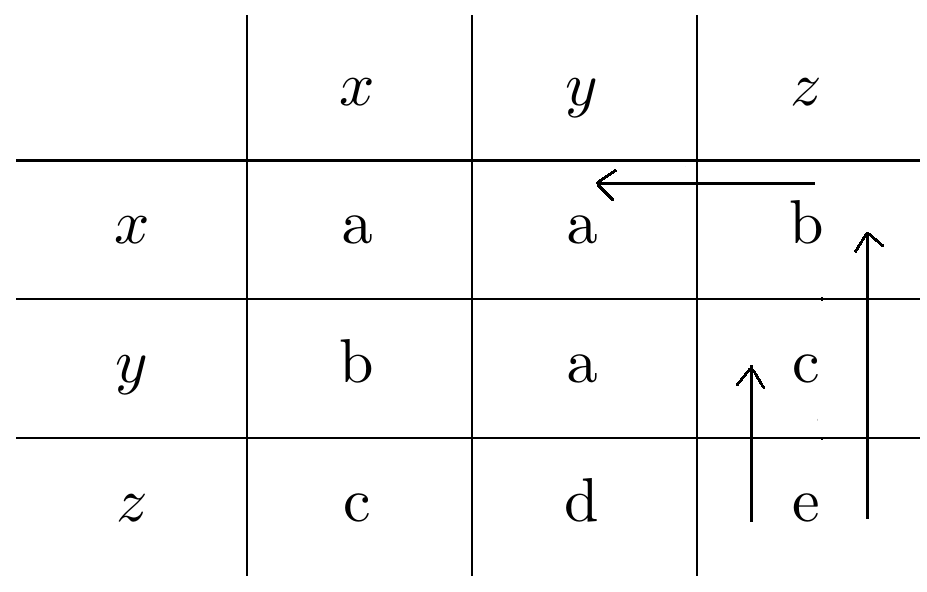
\includegraphics[width=0.70\textwidth]{gambar/isal2}}
	\caption{Contoh pembuatan table}
	\label{table latex}
\end{figure}

\noindent documentclass[10] \{ $article$ \} \par

\begin{itemize}
	\vspace{\baselineskip}
	\vspace{\baselineskip}
	\item Jadi class dokumen ini menggunaka kertas ukuran font 10 dan jenis dokumen nya itu artikel\par
\vspace{\baselineskip}
begin \{ $document$ \} \par
\vspace{\baselineskip}
	\item Memulai penulisan document\par
\vspace{\baselineskip}
begintitle\{ $table$ \} \par
\vspace{\baselineskip}
	\item Memulai untuk menggunakan table\par
\vspace{\baselineskip}
	\item Karena di dokumen ini membutuhkan table
	\vspace{\baselineskip}
\end{itemize}\par

\vspace{\baselineskip}
\begin{itemize}
	\item Jadi fungsi tabular itu untuk membuat kolom
\end{itemize}\par
\vspace{\baselineskip}
\begin{itemize}
	\item Tanda $ \vert $ itu untuk membuat garis kolomnya yang bisa kita tentukan sendiri\par
\vspace{\baselineskip}
	\item Dan tanda l itu adalah left
\end{itemize}\par

\vspace{\baselineskip}

\noindent Kesimpulan nya semua tulisan berada dikolom itu menggunakan rata kiri\par


\noindent hline\par

\vspace{\baselineskip}

\begin{itemize}
	\vspace{\baselineskip}
	\item Fungsi ini adalah membuat garis sesuai dengan lebar kolom yang kita buat\par
\vspace{\baselineskip}
	\item Hline ini juga berfungsi sebagai menentukan berapa baris yang kita mau
	\vspace{\baselineskip}
\end{itemize}\par

\begin{itemize}
\vspace{\baselineskip}
	\item Memasuki baris pertama yang di sebut attribute\par
\vspace{\baselineskip}
	\item Attribute ini adalah nama,npm,kelas,jurusan dan semester\par
\vspace{\baselineskip}
	\item Textbf ini berfungsi sebagaimembuat tulisan menjadi tebal atau bold\par
\vspace{\baselineskip}
	\item Tanda $\&$ ini berguna untuk memisahkan kolom satu dan kolom lain nya
	
\end{itemize}\par

\vspace{\baselineskip}
\noindent hline\par
\vspace{\baselineskip}

\begin{itemize}
	\item Berfungsi untuk membuat garis sesuai dengan lebar kolom yang kita buat\par

Garis pertama sudah di buat lalu buat garis kedua\par

Berarti kita masuk baris kedua\par

\vspace{\baselineskip}
Faisal akbar ramadhan$\&$1144010$\&$3DTID4$\&$TI$\&$7\par

Dibaris kedua ini tulisan faisal satu kolom dengan nama dan 3dtid4 satu kolom dengan attribute kelas, 1144010 ini berada di kolom npm, ti berada di kolom jurusan dan terakhir 7 adalah kolom untuk semester\par

\vspace{\baselineskip}
Selanjutnya isi table dengan cara yang sama dan isi table ini merupakan langkah berikutnya\par

\vspace{\baselineskip}
end \{ $tabular$ \} \par

\vspace{\baselineskip}
	\item Fungsinya untuk mengakhiri penggunaan tabular
\end{itemize}\par

\vspace{\baselineskip}
\noindent Karena sebelumnya kita telah menggunakan begin \{ $tabular$ \} \par


\noindent Maka harus diakhiri dengan end \{ $tabular$ \} \par


\noindent caption \{ $contoh table 1$ \} \par

\vspace{\baselineskip}
\noindent Untuk menambahkan keterangan dibawah table seperti contoh sebelumnya\par

\vspace{\baselineskip}
Contoh yang kita buat adalah contoh table 1\par

\vspace{\baselineskip}
\noindent end \{ table \} \par

\vspace{\baselineskip}
\begin{itemize}
	\item Fungsinya untuk mengakhiri penggunaan table\par
\vspace{\baselineskip}
Karena kita sebelumnya telah menggunakan begin \{ table \} \par

\vspace{\baselineskip}
Maka harus diakhiri dengan end \{ table \} \par

\vspace{\baselineskip}
end \{ document \} \par

\vspace{\baselineskip}
	\item Fungsinya untuk mengakhiri dokumen tersebut 
\end{itemize}\par


\vspace{\baselineskip}
\noindent Karena sebelumnya kita telah membuat begin$ \{ $document$ \} $\par


\noindent Maka diakhiri dengan end$ \{ $document$ \} $\par
\vspace{\baselineskip}
Setelah coding di tulis dengan tepat dan akurat setelah selesai jika pembaca ingin mengetahui hasil pembuatan table ini tinggal run di program tetapi projek ini sebelum dirun kita harus save nya terlebih dahulu sehingga bisa di jalan kan \par
\vspace{\baselineskip}
Setelah di pastikan projek disave lalu klik run build tersebut yang ada di atas file projek yang di buat\par
\vspace{\baselineskip}
Setelah run kita tunggu hasil dari pembuatan table tersebut maka akan keluar output yang sesuai anda buat \par
\vspace{\baselineskip}
Nama, npm, kelas dll telah sesuai tidak dengan nama yang telah di inputkan cek terlebih dahulu hasil output apabila ada kesalahan maka edit di codingan yang saat pembbuatan table nama pengisian nya seperti faisal akbar di ganti menjadi dimas rakasakti atau bebas apa yang anda ingin kan.\par

\vspace{\baselineskip}
apabila menginginkan table di buku yang anda buat masukan code tersebut tetapi dengan syarat jangan ada yang salah karena latex sensitive
 
\begin{equation}
Contoh :
\end{equation}

\vspace{\baselineskip}

\begin{itemize}
	\item Untuk baris baru\par

\vspace{\baselineskip}
begin \{ $table$ \} [h]\par

	\item Letak table nya ada bottom, top, dsb\par

\vspace{\baselineskip}
begin \{ $center$ \} \par

\vspace{\baselineskip}
	\item C itu center\par
\vspace{\baselineskip}
	\item R itu right\par
\vspace{\baselineskip}
	\item L itu left
\end{itemize}\par

\vspace{\baselineskip}
\vspace{\baselineskip}
\noindent hline\par

\begin{itemize}
	
	\item Ada beberapa perintah yang sering di gunakan karena wajib untuk table\par
\vspace{\baselineskip}
L\par

	\item Merupakan left kolom\par
\vspace{\baselineskip}
R\par

	\item Merupakan right kolom\par
\vspace{\baselineskip}
C\par

	\item Merupakan center kolom\par
\vspace{\baselineskip}
P\par

	\item Paraghraph kolom dengan lebar yang diinginkan\par
\vspace{\baselineskip}
\vspace{\baselineskip}
$ \vert $\par

	\item Garis vertical\par

$ \vert $$ \vert $\par

\vspace{\baselineskip}
Berarti dua garis vertical\par

\vspace{\baselineskip}
Setiap baris diakhiri dengan symbol \par
\vspace{\baselineskip}
Untuk memisahkan kolom menggunakan $\&$\par
\vspace{\baselineskip}
Garis vertical serebar table menggunakan perintah hline\par
\vspace{\baselineskip}
Menyisipkan kode $ \vert $ pada kolom\par

\vspace{\baselineskip}
	\item Sedangkan horizontal menggunakan perintah cline\par

H\par

\vspace{\baselineskip}
	\item Table diletakan persis di tempat perintah tsb dituliskan\par

T\par

	\item Table dituliskan di bagian atas halaman\par

\vspace{\baselineskip}
B\par

	\item Table diletakan di bagian bawah halaman\par 

\vspace{\baselineskip}
p\par
\end{itemize}

\begin{verbatim}
	
1.3 Table diletakan pada halaman khusus yang hanya memuat table itu sendiri

begin \{ table \} [htbp]
begin \{ center \} 
caption \{ Contoh 1 \} 

begin \{ tabular \}

hline

 Nama $\&$ Negara $\&$ Club

hline

  Ronaldo $\&$ Brazil $\&$ Real Madrid 

  Lionel Messi $\&$ Argentina $\&$ Barcelona

hline\par

end \{ tabular \} 

end \{ center \} 

end \{ table \} 

end \{ document \} 

\end{verbatim}

\vspace{\baselineskip}
\subsection{Berikut adalah pengantar cara penulisan dengan benar menurut para ahli}

\vspace{\baselineskip}

Agar pembaca tujuan nya mengetahui tujuan pembuatan table pada karya ilmiah atau buku dan lain lain\par

\vspace{\baselineskip}

\begin{itemize}
	\item Teknik menulis karya ilmiah seperti laporan penelitian dosen, buku, dan artikel jurnal ilmiah dapat disertai dengan tabel dan gambar. Tabel berguna untuk menyajikan data secara ringkas dalam bentuk matriks. Demikian juga gambar, yang dapat berupa foto, peta, bagan alir, sebenarnya juga merupakan data dalam bentuk visual.\par

\vspace{\baselineskip}
	\item Tabel dan gambar, kalau digunakan dengan benar, selain berguna untuk menyajikan data, juga menjadikan karya ilmiah tampil lebih menarik. Hanya saja tentu ada catatannya, keduanya ditampilkan sesuai dengan persyaratan pencantuman tabel dan gambar dalam karya ilmiah.\par

\vspace{\baselineskip}
	\item Sayangnya, banyak dosen dan mahasiswa mencantumkan tabel dan gambar apa adanya. Akibatnya, bukan menjadikan buku atau karya ilmiah menjadi lebih mudah dimengerti, lebih menarik, tetapi justru sebaliknya. Jangan sampai tabel dan gambar sulit dimengerti sehingga membingungkan. Bisa jadi tabel dan gambar yang tampil sekenanya justru menjadikan tampilan buku berantakan. Kemampuan menyajikan tabel penting dalam teknik menulis buku atau karya ilmiah\par

\vspace{\baselineskip}
	\item Menampilkan tabel dan gambar dalam buku, perlu terlebih dahulu memperhatikan gaya penulisan ilmiah yang akan digunakan. Bila akan menggunakan gaya penulisan APA, maka perlu diikuti aturan pencantuman tabel dan pencantuman gambar menurut gaya tersebut. Beberapa ketentuan yang perlu diperhatikan antara lain, ukuran tabel dan gambar tidak boleh melewati batas tepi halaman.\par

\vspace{\baselineskip}
	\item Tabel dan gambar harus disertai dengan judul yang masing-masing didahului dengan tulisan ‘Tabel x’ dan ‘Gambar x’, di mana x merupakan nomor urut. Judul ditulis dengan hanya huruf awal kata pertama dan huruf awal kata-kata benda nama diri yang ditulis kapital (bukan huruf awal setiap kata) dan bukan menggunakan huruf tebal atau miring.\par

\vspace{\baselineskip}
	\item Setiap tabel atau gambar harus dirujuk dalam teks tulisan sebagaimana merujuk pustaka dengan mencantumkan Tabel x atau Gambar x. Tabel harus diberi kepala kolom dan kepala baris yang jelas dengan cara penulisan sebagaimana penulisan judul tabel. Bila isi tabel merupakan hasil pengukuran maka satuan dicantumkan sebagai bagian dari judul kolom.

\end{itemize}\par

\vspace{\baselineskip}
\subsection{Aturan Aturan pembuatan table}

\vspace{\baselineskip}

Dalam sebuah table biasana terdiri dari beberapa baris dan beberapa kolom.\par

\vspace{\baselineskip}

Dalam hal ini, untuk membuat sebuah table yang benar diperlukan aturan-aturan sebagai berikut:\par

\vspace{\baselineskip}

\noindent Judul table\par


\noindent Dalam judul table harus diperhatikan hal-hal sebagai berikut:\par

\begin{itemize}
	\vspace{\baselineskip}
	\item harus ditulis ditengah tengah bagian teratas\par

\vspace{\baselineskip}
	\item diberi nomor agar lebih mudah dalam pencarian table biasanya nomor itu meliputi bab berapa materi itu sedang di bahas dan nomor urut table itu sendiri.
	
\end{itemize}\par

\vspace{\baselineskip}
\noindent Contoh daftar 1(2) artinya table itu membahas materi bab1 dan urutan table ke dua yang di bahas\par

\begin{itemize}
\vspace{\baselineskip}
	\item ditulis dengan huruf besar semua\par
\vspace{\baselineskip}
	\item Ditulis secara singkat dan jelas meliputi: masalah apa, dimana masalah itu terjadi, kapan masalah itu terjadi dan satuan dari objek yang di permasalahkan\par
\vspace{\baselineskip}
	\item Ditulis dalam berupa baris dengan tiap barisnya menggambarkan sebuah kalimat yang lengkap\par
\vspace{\baselineskip}
	\item Sebaliknya tiap baris jangan dilakukan pemisahan kata
\end{itemize}\par
\vspace{\baselineskip}
\vspace{\baselineskip}

\noindent Contoh:\par


\noindent Daftar 1(1)\par

\vspace{\baselineskip}

\noindent BERAT BADAN MAHASISWA PROGRAM S-1 PENDIDIKAN GURU SEKOLAH DASAR DICATAT DALAM KG\par

\vspace{\baselineskip}
\noindent Judul baris\par

\begin{itemize}
\vspace{\baselineskip}
	\item Ditulis secara singkat dan jelas \par
\vspace{\baselineskip}
	\item Dapat ditulis dalam beberapa baris\par
\vspace{\baselineskip}
	\item Sebaliknya jangan dilakukan pemisahan bagian kata
\end{itemize}\par

\vspace{\baselineskip}
\noindent Judul kolom\par

\begin{itemize}
	\vspace{\baselineskip}
	\item Ditulis secara singkat dan jelas\par
\vspace{\baselineskip}
	\item Dapat ditulis dalam beberapa baris\par
\vspace{\baselineskip}
	\item Sebaliknya jangan dilakukan pemisahan bagian kata
\end{itemize}\par

\vspace{\baselineskip}

Disebelah kiri bawah table biasanya terdapat bagian untuk menuliskan catatan yang diberikan atau bisa juga kata sumber yang menjelaskan dari mana data itu dikutif. \par 

\vspace{\baselineskip}
Jika kata sumber itu tidak ada ini berarti bahwa pemakai data itu sendiri yang mengumpulkan datanya bisa berupa data fiktif atau data yang benar benar hasil penelitiannya\par

\vspace{\baselineskip}

\noindent 2.3 Jika ada data mengenai waktu, maka waktu hendaknya di susun berurutan\par

\vspace{\baselineskip}
\noindent Contoh\par

\vspace{\baselineskip}
Senin, selasa dan seterusnya\par
\vspace{\baselineskip}
2000, 2001 dan seterusnya\par
\vspace{\baselineskip}
Januari, febuari dan seterusnya\par

\vspace{\baselineskip}

\noindent 2.4 Jika ada data mengenai kategori maka kategori disusun menurut kebiasaan\par

\vspace{\baselineskip}
\noindent Contoh\par

\vspace{\baselineskip}

Laki-laki dahulu kemudian perempuan\par

\vspace{\baselineskip}
Besar dulu setelah itu kecil\par

\vspace{\baselineskip}
Untung dahulu baru rugi \par

\vspace{\baselineskip}
Bagus dulu setelah itu jelek\par

Contoh pembuatan tabel :
\begin{table}[ht]
	\caption{Dokumentasi Paket}
	\centering
	\begin{tabular}{cccc}
		\hline
		No&Isi\\
		\hline
		1&Adding Footnose&\\
		2&Create Table&\\
		\hline
	\end{tabular}
\end{table}
